\documentclass[11pt,class=report,crop=false]{standalone}
\usepackage[screen]{../python}


\begin{document}

% Pour latitude/longitude 3d
% Stereographic and cylindrical map projections
% Author: Tomasz M. Trzeciak
% Source: LaTeX-Community.org
%         <http://www.latex-community.org/viewtopic.php?f=4&t=2111>

\newcommand\pgfmathsinandcos[3]{%
  \pgfmathsetmacro#1{sin(#3)}%
  \pgfmathsetmacro#2{cos(#3)}%
}
\newcommand\LongitudePlane[3][current plane]{%
  \pgfmathsinandcos\sinEl\cosEl{#2} % elevation
  \pgfmathsinandcos\sint\cost{#3} % azimuth
  \tikzset{#1/.style={cm={\cost,\sint*\sinEl,0,\cosEl,(0,0)}}}
}
\newcommand\LatitudePlane[3][current plane]{%
  \pgfmathsinandcos\sinEl\cosEl{#2} % elevation
  \pgfmathsinandcos\sint\cost{#3} % latitude
  \pgfmathsetmacro\yshift{\cosEl*\sint}
  \tikzset{#1/.style={cm={\cost,0,0,\cost*\sinEl,(0,\yshift)}}} %
}
\newcommand\DrawLongitudeCircle[2][1]{
  \LongitudePlane{\angEl}{#2}
  \tikzset{current plane/.prefix style={scale=#1}}
   % angle of "visibility"
  \pgfmathsetmacro\angVis{atan(sin(#2)*cos(\angEl)/sin(\angEl))} %
  \draw[current plane] (\angVis:1) arc (\angVis:\angVis+180:1);
  \draw[current plane,dashed] (\angVis-180:1) arc (\angVis-180:\angVis:1);
}
\newcommand\DrawLatitudeCircle[2][1]{
  \LatitudePlane{\angEl}{#2}
  \tikzset{current plane/.prefix style={scale=#1}}
  \pgfmathsetmacro\sinVis{sin(#2)/cos(#2)*sin(\angEl)/cos(\angEl)}
  % angle of "visibility"
  \pgfmathsetmacro\angVis{asin(min(1,max(\sinVis,-1)))}
  \draw[current plane] (\angVis:1) arc (\angVis:-\angVis-180:1);
  \draw[current plane,dashed] (180-\angVis:1) arc (180-\angVis:\angVis:1);
}


% \begin{tikzpicture} % "THE GLOBE" showcase
% \def\R{2.5} % sphere radius
% \def\angEl{35} % elevation angle
% \filldraw[ball color=white] (0,0) circle (\R);
% \foreach \t in {-80,-60,...,80} { \DrawLatitudeCircle[\R]{\t} }
% \foreach \t in {-5,-35,...,-175} { \DrawLongitudeCircle[\R]{\t} }
% \end{tikzpicture}

%====================================================================
\chapitre{Images 3D}
%====================================================================

\objectifs{Comment dessiner des objets dans l'espace et comment les représenter sur un plan ?}


\bigskip

%%%%%%%%%%%%%%%%%%%%%%%%%%%%%%%%%%%%%%%%%%%%%%%%%%%%%%%%%%%%%%%%
%%%%%%%%%%%%%%%%%%%%%%%%%%%%%%%%%%%%%%%%%%%%%%%%%%%%%%%%%%%%%%%%

\begin{cours}[Images 3D avec matplollib]

\index{image}
\index{module!matplotlib@\ci{matplolib}}

Avec le module \ci{matplolib} il est assez facile de tracer une représentation des objets dans l'espace.
Le principe est similaire à l'affichage dans le plan, sauf bien sûr qu'il faut préciser trois coordonnées $x,y,z$ pour déterminer un point de l'espace.

\bigskip

Voici un code très simple qui affiche :
\begin{itemize}
	\item un point \couleurnb{bleu }{}de coordonnées $(2,1,3)$,
	\item des segments \couleurnb{rouges }{}qui relient les points de la liste  $(0,0,0)$, $(1,2,3)$, $(4,5,6)$, $(3,5,0)$.
\end{itemize}

\begin{center}
	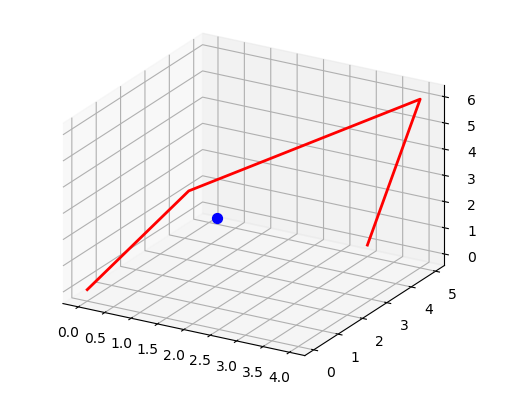
\includegraphics[scale=\myscale,scale=0.3]{ecran-images3d-cours1}
	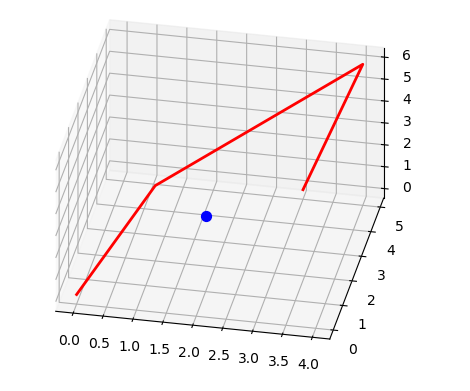
\includegraphics[scale=\myscale,scale=0.3]{ecran-images3d-cours2}
	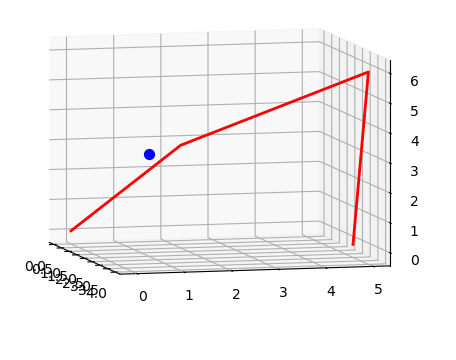
\includegraphics[scale=\myscale,scale=0.3]{ecran-images3d-cours3}	
\end{center}

Une fenêtre s'affiche dans laquelle sont dessinés le point et les segments ainsi que les plans quadrillés de coordonnées. L'image est dynamique : à l'aide de la souris tu peux faire tourner le dessin afin de changer de point de vue.

\begin{lstlisting}
import matplotlib.pyplot as plt
from mpl_toolkits.mplot3d import Axes3D

# Initialisation
fig = plt.figure()
ax = fig.gca(projection='3d',proj_type = 'ortho') 

# Affichage d'un point
x,y,z = (2,1,3)
ax.scatter(x,y,z,color='blue',s=50)

# Segments reliant des points
points  = [(0,0,0),(1,2,3),(4,5,6),(3,5,0)]
liste_x = [x for x,y,z in points]
liste_y = [y for x,y,z in points]
liste_z = [z for x,y,z in points]

ax.plot(liste_x,liste_y,liste_z,color='red',linewidth=2)

# Affichage
plt.show()
\end{lstlisting}


\emph{Avertissement.} Pour afficher des segments la commande \ci{plot} n'est pas très naturelle (mais c'était déjà le cas dans le plan). Par exemple pour relier le point $(1,2,3)$ au point $(4,5,6)$ on donne d'abord la liste des $x$, puis la liste des $y$, puis la liste des $z$ :
\mycenterline{\ci{plot([1,4],[2,5],[3,6])}}

\end{cours}


%%%%%%%%%%%%%%%%%%%%%%%%%%%%%%%%%%%%%%%%%%%%%%%%%%%%%%%%%%%%%%%%
%%%%%%%%%%%%%%%%%%%%%%%%%%%%%%%%%%%%%%%%%%%%%%%%%%%%%%%%%%%%%%%%

\begin{cours}[Surface d'équation $z=f(x,y)$]
\sauteligne
\begin{itemize}
	\item Une \defi{fonction de deux variables} associe à un couple de réels $(x,y)$ un réel $f(x,y)$, c'est donc une fonction $f : \Rr^2 \to \Rr$, $(x,y) \mapsto f(x,y)$.
	
	\item Le \defi{graphe} d'une fonction de deux variables est la surface d'équation $z=f(x,y)$, autrement dit 
	c'est 
	$$\big\{ (x,y,z) \in \Rr^3 \mid z = f(x,y) \big\}$$
	
	\item Pour tracer le graphe d'une fonction d'une seule variable, on relie des points $(x,f(x))$ entre eux (sur la figure de gauche $5$ points), si les points sont suffisamment proches, la courbe a l'air lisse (sur la figure de droite avec $20$ points).
\myfigure{0.8}{
\tikzinput{fig-surface-1}\qquad\qquad
\tikzinput{fig-surface-2}
}

\myfigure{0.8}{\tikzinput{fig-surface-3}}	
	
	\item Pour tracer une surface associée à une fonction de deux variables on commence par quadriller le plan $(x,y)$.
	
	\myfigure{0.4}{\tikzinput{fig-surface-4}}	
	
	\item Ensuite on trace les points $(x,y,f(x,y))$ au-dessus de chaque ligne verticale\couleurnb{ bleue}{} du plan en les reliant puis on fait la même chose sur chaque ligne horizontale\couleurnb{ rouge}{}.

\begin{center}
	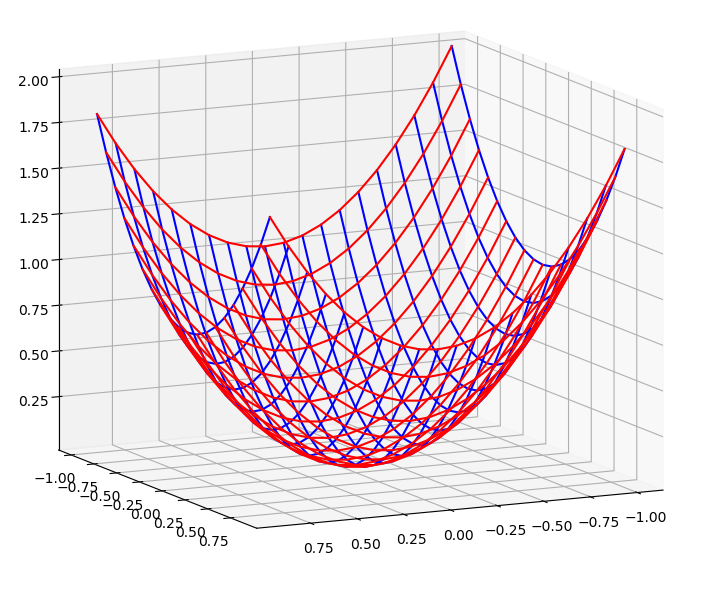
\includegraphics[scale=\myscale,scale=0.3]{ecran-surface-1}
\end{center}	
\end{itemize}	
	
\end{cours}


%%%%%%%%%%%%%%%%%%%%%%%%%%%%%%%%%%%%%%%%%%%%%%%%%%%%%%%%%%%%%%%%
% Activité 1 - Surfaces
%%%%%%%%%%%%%%%%%%%%%%%%%%%%%%%%%%%%%%%%%%%%%%%%%%%%%%%%%%%%%%%%

\begin{activite}[Surfaces]

	\objectifs{Objectifs : tracer la surface d'équation $z = f(x,y)$ donnée par une fonction de deux variables.}

\begin{center}
	\begin{minipage}{0.4\textwidth}
		\begin{center}
			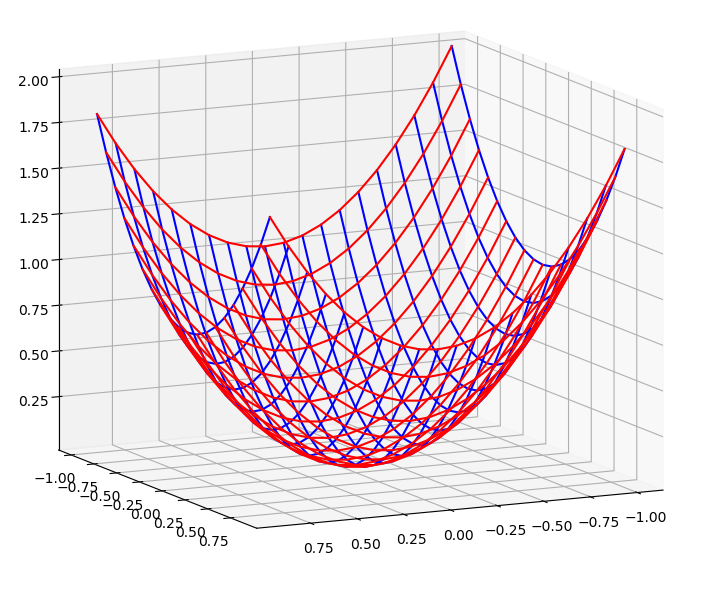
\includegraphics[scale=\myscale,scale=0.3]{ecran-surface-1}
			
			Bol -- $f(x,y) = x^2+y^2$
		\end{center}
	\end{minipage}\quad
	\begin{minipage}{0.4\textwidth}
		\begin{center}
			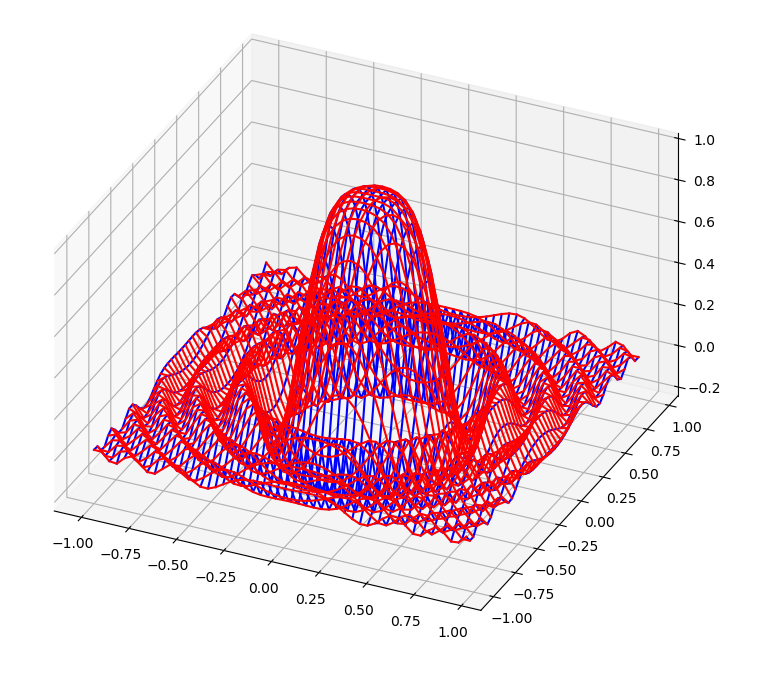
\includegraphics[scale=\myscale,scale=0.3]{ecran-surface-2}
			
			Goutte qui tombe dans l'eau -- $f(x,y) = \frac{\sin(r)}{r}$ où
			$r = 20(x^2+y^2)$
		\end{center}
	\end{minipage}
\end{center}

\begin{enumerate}
	
	\item Programme une fonction \ci{f(x,y)} qui renvoie une valeur en fonction de $x$ et de $y$.
	Voici des exemples de fonctions :
	\begin{itemize}
		\item  $f(x,y) = x^2+y^2$ \quad (un bol).
		\item $f(x,y) = \frac{\sin(r)}{r}$ où $r = 20(x^2+y^2)$ \quad  (une goutte qui tombe dans l'eau).
		\item $f(x,y) = \sin(10x)+\cos(10y)$ \quad (une boîte d'\oe ufs).
		\item $f(x,y) = x^2-y^2$ \quad (une selle de cheval).
		\item $f(x,y) = \exp(-\frac13x^3+x-y^2)$ \ \  pour $x \in [-2,3]$ et $y \in [-2.5,2.5]$ \  (un sommet et un col).
	\end{itemize}
	Les graphes d'équation $z=f(x,y)$ sont dessinés ci-dessus ou ci-dessous. \`A l'exception de la dernière fonction, les tracés sont obtenus pour $x \in[-1,+1]$ et $y \in [-1,+1]$.

\begin{center}
	\begin{minipage}{0.3\textwidth}
		\begin{center}
			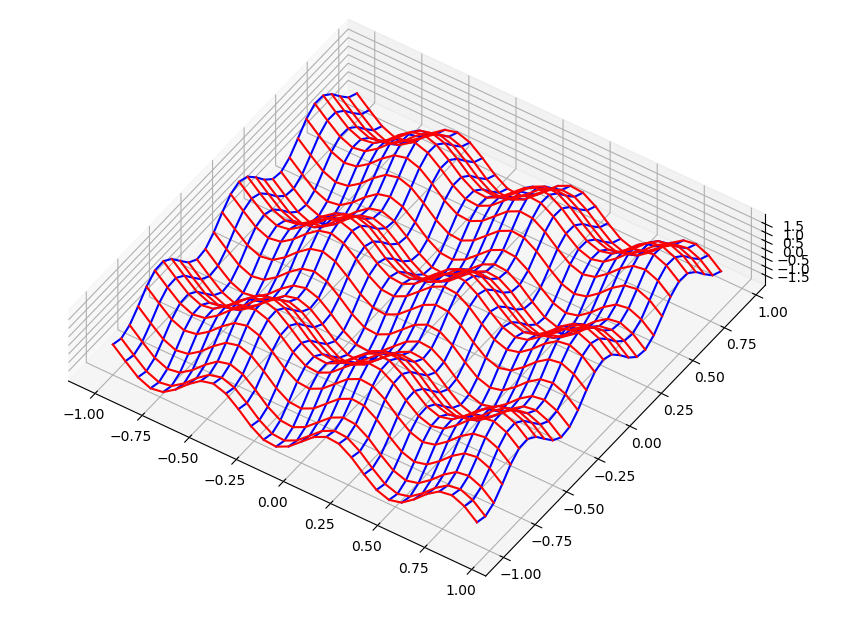
\includegraphics[scale=\myscale,scale=0.2]{ecran-surface-3}
			
			Boîte d'\oe ufs -- $f(x,y) = \sin(10x)+\cos(10y)$
		\end{center}
	\end{minipage}\quad
	\begin{minipage}{0.3\textwidth}
		\begin{center}
			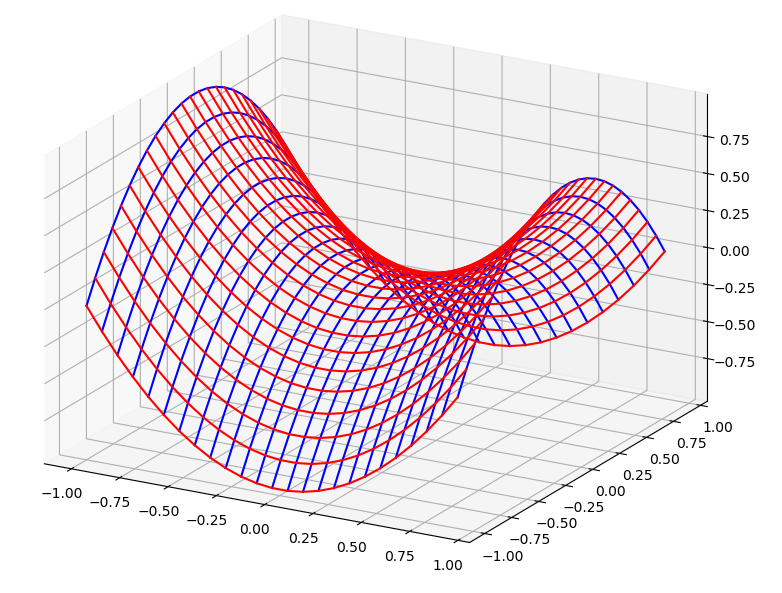
\includegraphics[scale=\myscale,scale=0.2]{ecran-surface-4}
			
			Selle de cheval -- $f(x,y) = x^2-y^2$
		\end{center}
	\end{minipage}
	\begin{minipage}{0.3\textwidth}
		\begin{center}
			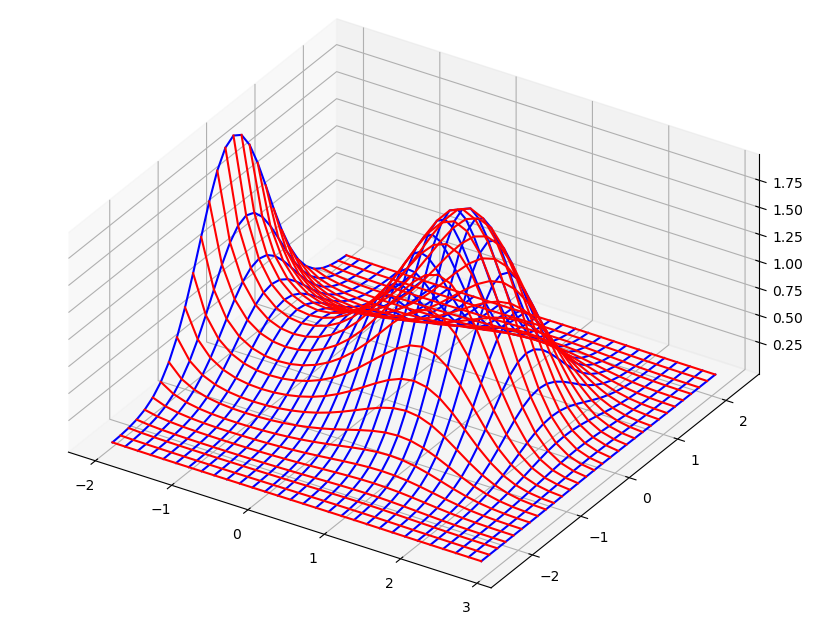
\includegraphics[scale=\myscale,scale=0.2]{ecran-surface-5}
			
			Sommet et col -- $f(x,y) = \exp(-\frac13x^3+x-y^2)$ pour $x \in [-2,3]$ et $y \in [-2.5,2.5]$
		\end{center}
	\end{minipage}
\end{center}	
	
	\item 
	\begin{enumerate}
		\item Définis des constantes globales \ci{xmin = -1},  \ci{xmax = +1} pour définir l'intervalle $x\in[-1,+1]$ et \ci{ymin = -1},  \ci{ymax = +1} pour définir l'intervalle $y\in[-1,+1]$.
		
		Définis aussi une constante globale \ci{nbpoints = 10} qui correspond au nombre $N$ de découpages. Chaque ligne est formée de $N+1$ points ; il y a aussi en tout $N+1$ lignes tracées dans chaque direction.
		
		\item Programme une fonction \ci{liste_points_xcst(x)} 
		qui renvoie une liste de points $(x,y,z)$ où :
		\begin{itemize}
			\item $x$ est la valeur donnée en paramètre de la fonction,
			\item $y$ prend les valeurs $y_{\min} + k h$ pour $k=0,1,\ldots,N$ et $h = \frac{y_{\max}-y_{\min}}{N}$ (on rappelle que $N = $ \ci{nbpoints}),
			\item $z = f(x,y)$.
		\end{itemize}
	
		Par exemple pour la fonction $f(x,y)=x^2+y^2$, $x=0$ et l'intervalle $[-1,+1]$ des $y$ découpé en $N=5$ morceaux, la liste des points renvoyée est une liste de $N+1=6$ points :		
		\mycenterline{\ci{[(0, -1, 1), (0, -0.6, 0.36), (0, -0.2, 0.04),}}
		\mycenterline{\ci{(0, 0.2, 0.04), (0, 0.6, 0.36), (0, 1, 1)]}}
		
		
		\item Fais le même travail pour une fonction \ci{liste_points_ycst(y)} où cette fois $y$ est fixé et c'est $x$ qui varie.
	\end{enumerate}

	\item
	\begin{enumerate}
	  \item Programme une fonction \ci{trace_ligne(liste_points)} (ou mieux \ci{trace_ligne(liste_points,couleur='gray')} permettant de changer la couleur du trait) qui relie les points $(x,y,z)$ de la liste par des segments (du premier au dernier).
	
	  Voici l'affichage des $6$ points de la liste de la question précédente.
	  \begin{center}
	  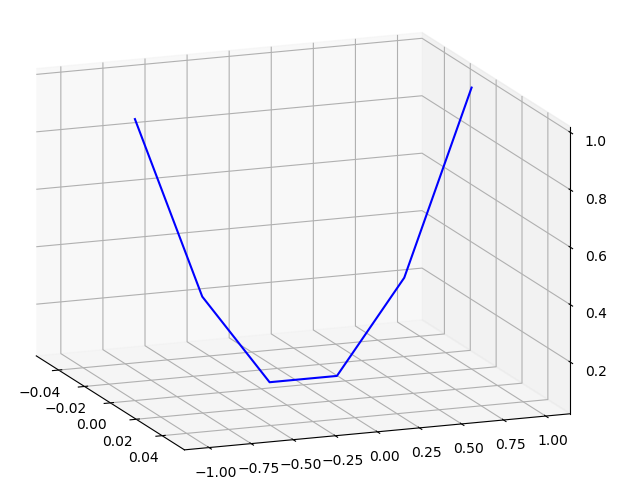
\includegraphics[scale=\myscale,scale=0.2]{ecran-surface-6}
	  \end{center}

	  \item Programme ensuite une fonction \ci{trace_surface()} qui dessine la surface en traçant $N+1$ lignes \couleurnb{(bleues)}{} pour chacune desquelles $x$ est constant (figure de gauche) et aussi $N+1$ lignes \couleurnb{(rouges)}{} pour chacune desquelles $y$ est constant (figure du milieu) pour obtenir une représentation de la surface (figure de droite). 
	  
	  \begin{center}
	  	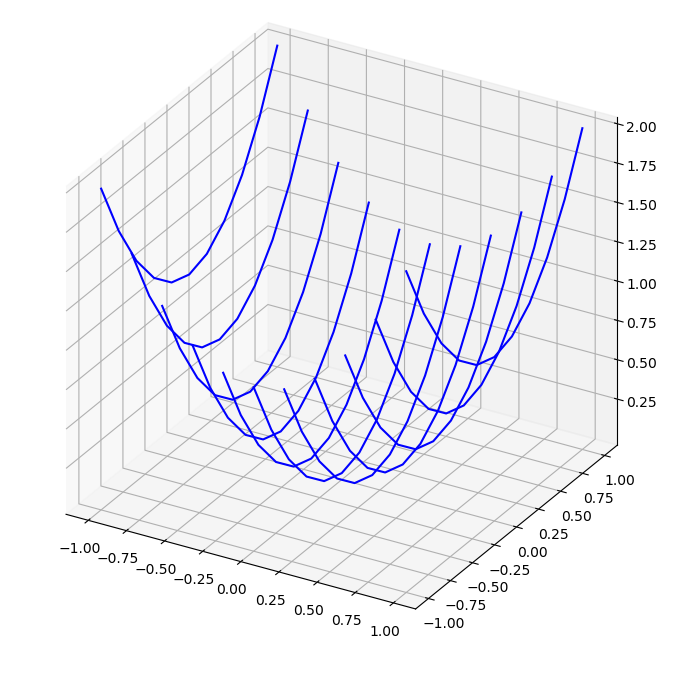
\includegraphics[scale=\myscale,scale=0.2]{ecran-surface-7}
	  	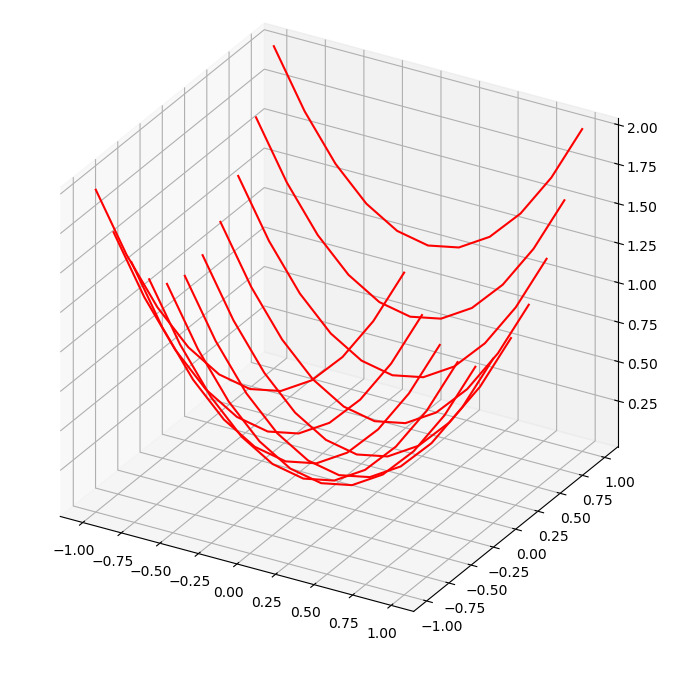
\includegraphics[scale=\myscale,scale=0.2]{ecran-surface-8}
	  	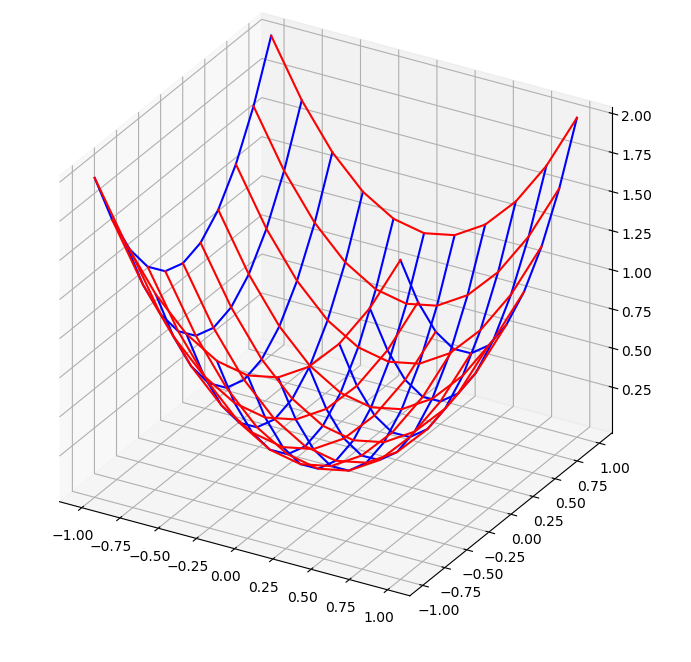
\includegraphics[scale=\myscale,scale=0.2]{ecran-surface-9}
	  \end{center}
	\end{enumerate}
\end{enumerate}



\end{activite}




%%%%%%%%%%%%%%%%%%%%%%%%%%%%%%%%%%%%%%%%%%%%%%%%%%%%%%%%%%%%%%%%
%%%%%%%%%%%%%%%%%%%%%%%%%%%%%%%%%%%%%%%%%%%%%%%%%%%%%%%%%%%%%%%%

\begin{cours}[Perspective]
	
Ceci n'est pas un cube !

\myfigure{1.2}{\tikzinput{fig-perspective-1}}  

C'est juste une union de segments du plan. Notre cerveau est capable de reconstruire un objet en trois dimensions à partir d'un image plane.
Pour dessiner sur une feuille un objet 3D il faut donc une formule qui transforme un point $(x,y,z)$ de l'espace en un point $(X,Y)$ du plan.
Il existe différentes formules, en voici quelques unes. Pour les dessins voir l'activité qui suit.

\bigskip
\textbf{Perspective cavalière.}

Elle est définie par une constante $k$ qui réduit les longueurs des segments obliques et un angle $\alpha$.
\myfigure{1}{\tikzinput{fig-perspective-3}}  

$$\left\{
\begin{array}{rcl}
X &=& x + k \cos(\alpha)y \\
Y &=& z + k \sin(\alpha)y
\end{array}
\right.$$



Les constantes $\alpha$ et $k$ sont le plus souvent  $(\alpha=\frac\pi4,k=\frac12)$ ou bien $(\alpha=\frac\pi6,k=0.7)$.
 
\bigskip

\textbf{Perspective axonométrique.}

Cette opération consiste à tourner d'abord l'objet selon deux axes (il y a donc deux angles $\omega$ et $\alpha$), avant de projeter sur un plan.

$$\left\{
\begin{array}{rcl}
X &=& \cos(\omega)x - \sin(\omega)y \\
Y &=& -\sin(\omega)\sin(\alpha)x - \cos(\omega)\sin(\alpha)y + \cos(\alpha)z
\end{array}
\right.$$ 

Où $\omega$ et $\alpha$ sont des angles fixés. Dans le cas particulier $\omega=0.61$ et $\alpha=\frac\pi4$
on obtient la \emph{perspective isométrique}.
 
\bigskip

\textbf{Perspective conique.} 

Il s'agit de regarder un objet de l'espace depuis un point $(0,-f,0)$ et de le projeter sur le plan $(y=0)$ ; $f$ est une valeur constante qui s'appelle la \emph{focale}.

\myfigure{0.5}{\tikzinput{fig-perspective-2}}  

Les formules sont :
$$\left\{
\begin{array}{rcl}
X &=& kx \\
Y &=& kz
\end{array}
\right.  \qquad \text{ avec } \quad k = \frac{f}{y+f}.$$ 
	
\end{cours}



%%%%%%%%%%%%%%%%%%%%%%%%%%%%%%%%%%%%%%%%%%%%%%%%%%%%%%%%%%%%%%%%
% Activité 2 - Perspective
%%%%%%%%%%%%%%%%%%%%%%%%%%%%%%%%%%%%%%%%%%%%%%%%%%%%%%%%%%%%%%%%

\begin{activite}[Perspective]
	
\index{perspective}
	
\objectifs{Objectifs : transformer un objet de l'espace en un objet du plan afin de l'afficher.}


Pour les exemples on va afficher différentes projections du cube donné par les coordonnées suivantes :
\mycenterline{\ci{cube  = [(0,0,0),(1,0,0),(1,1,0),(0,1,0),(0,0,1),(1,0,1),(1,1,1),(0,1,1)]}}

\begin{enumerate}
	
	\item Programme une fonction \ci{affiche_cube_3d(cube)} qui à partir d'une liste de $8$ points $[P_0,P_1,\ldots,P_7]$
	trace l'affichage 3D du cube $(P_0,P_1,\ldots,P_7)$. Il s'agit juste de tracer les $12$ arêtes du cube !
	
	\begin{center}
		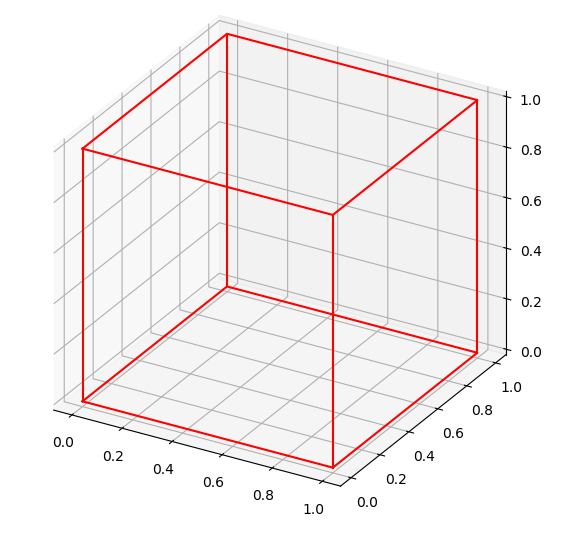
\includegraphics[scale=\myscale,scale=0.4]{ecran-perspective-1}
	\end{center}

	\item \textbf{Perspective cavalière.}
	\begin{enumerate}
		\item Programme une fonction \ci{perspective_cavaliere(P)} (ou mieux \ci{perspective_cavaliere(P,alpha=pi/4,k=0.5)})
		qui à partir d'un point $P$ de l'espace de coordonnées $(x,y,z)$ renvoie le point $Q$ du plan de coordonnées $(X,Y)$ selon la formule :
		$$\left\{
		\begin{array}{rcl}
		X &=& x + k \cos(\alpha)y \\
		Y &=& z + k \sin(\alpha)y
		\end{array}
		\right.$$
		
		Pour les constantes $\alpha$ et $k$, on testera $(\alpha=\frac\pi4,k=\frac12)$ puis $(\alpha=\frac\pi6,k=0.7)$.
	
		\item Programme une fonction \ci{affiche_cube_2d(cube2d)} qui à partir d'une liste $[Q_0,Q_1,\ldots,Q_7]$
		de $8$ \textbf{points du plan}, relie les points deux à deux comme si c'était les arêtes d'un cube.
	
		\item \`A partir des sommets du cube 3D $(P_0,P_1,\ldots,P_7)$, calcule sa projection $(Q_0,Q_1,\ldots,Q_7)$ dans le plan et affiche cette projection du cube. Voici le résultat ci-dessous : il s'agit bien ici de deux images du plan !
		
		\begin{center}
		\begin{minipage}{0.45\textwidth}
		\begin{center}
			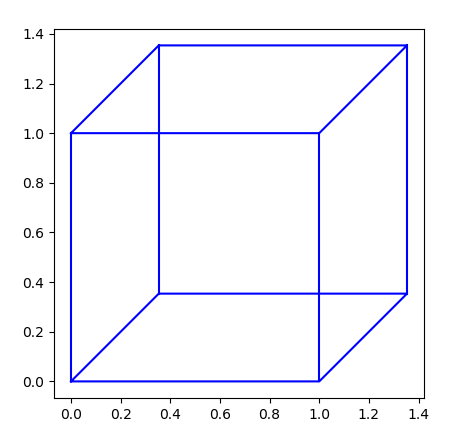
\includegraphics[scale=\myscale,scale=0.4]{ecran-perspective-2}
		
			$\alpha=\frac\pi4$, $k=\frac12$
		\end{center}
		\end{minipage}
		\begin{minipage}{0.45\textwidth}
		\begin{center}
		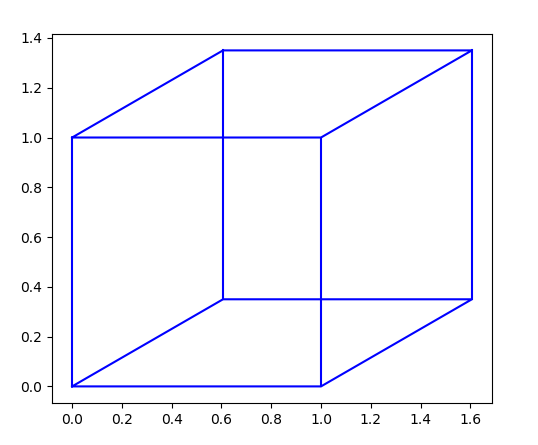
\includegraphics[scale=\myscale,scale=0.4]{ecran-perspective-3}
		
		$\alpha=\frac\pi6$, $k=0.7$
		\end{center}
		\end{minipage}
		\end{center}
	
	
				
	\end{enumerate}	
	
   \item \textbf{Perspective axonométrique.}
    Fais le même travail pour une fonction \ci{perspective_axonometrique(P)}
   (ou mieux  \ci{perspective_axonometrique(P, alpha=0.61, omega=pi/4)})
   qui pour $P = (x,y,z)$ point de l'espace renvoie le point $Q = (X,Y)$ du plan suivant les formules :
   $$\left\{
   \begin{array}{rcl}
   X &=& \cos(\omega)x - \sin(\omega)y \\
   Y &=& -\sin(\omega)\sin(\alpha)x - \cos(\omega)\sin(\alpha)y + \cos(\alpha)z
   \end{array}
   \right.$$
   
   Affiche la projection du cube.
   
	\begin{center}
	\begin{minipage}{0.45\textwidth}
	\begin{center}
		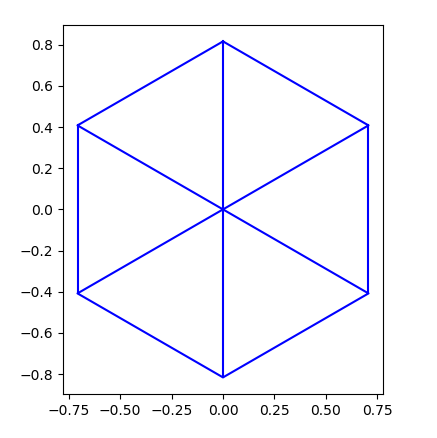
\includegraphics[scale=\myscale,scale=0.4]{ecran-perspective-4}
			
		Perspective isométrique : $\omega=0.61$, $\alpha=\frac\pi4$
	\end{center}
	\end{minipage}
	\begin{minipage}{0.45\textwidth}
	\begin{center}
		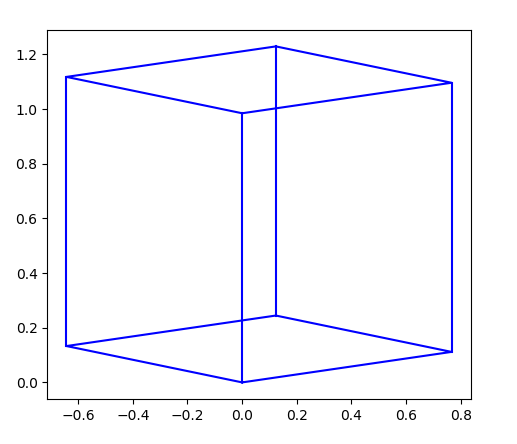
\includegraphics[scale=\myscale,scale=0.4]{ecran-perspective-5}
			
		Perspective axonométrique avec $\omega=30^\circ$, $\alpha=-10^\circ$ (à convertir en radians)
	\end{center}
	\end{minipage}
	\end{center}

	Avec la perspective isométrique (à gauche) toutes les arêtes projetées ont la même longueur. Ici la projection n'est pas très lisible car deux sommets sont projetés sur le même point.
  
  
   \item \textbf{Perspective conique.} 
   Fais le même travail pour une fonction \ci{perspective_conique(P)}
   (ou mieux  \ci{perspective_conique(P,f=2)}) qui pour $P = (x,y,z)$ point de l'espace renvoie le point 
   $Q = (X,Y)$ du plan suivant les formules :
   $$\left\{
	\begin{array}{rcl}
	X &=& kx \\
	Y &=& kz
	\end{array}
	\right.  \qquad \text{ avec } \quad k = \frac{f}{y+f}.$$ 
	
	Voici l'affichage du cube :
	\mycenterline{\ci{cube  = [(1,1,-1),(2,1,-1),(2,2,-1),(1,2,-1),(1,1,-2),(2,1,-2),(2,2,-2),(1,2,-2)]}}
	pour différentes valeurs de la focale $f$.
	\begin{center}
	\begin{minipage}{0.2\textwidth}
	\begin{center}
		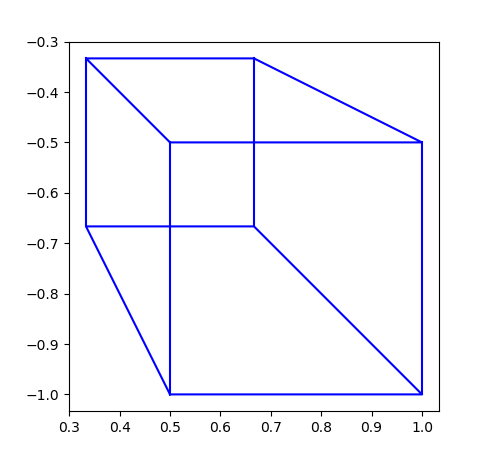
\includegraphics[scale=\myscale,scale=0.25]{ecran-perspective-6-1}
			
		$f=1$
	\end{center}
	\end{minipage}
	\begin{minipage}{0.2\textwidth}
	\begin{center}
		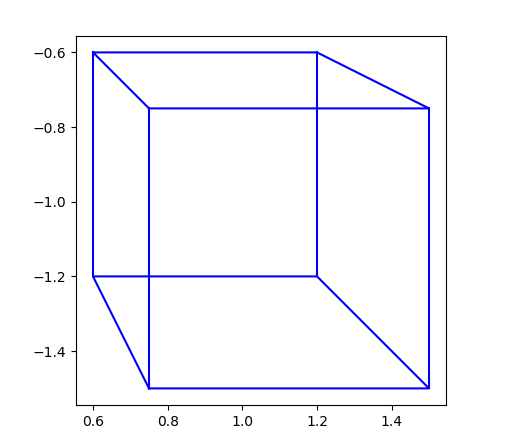
\includegraphics[scale=\myscale,scale=0.25]{ecran-perspective-6-3}
		
		$f=3$
	\end{center}
	\end{minipage}
	\begin{minipage}{0.2\textwidth}
	\begin{center}
		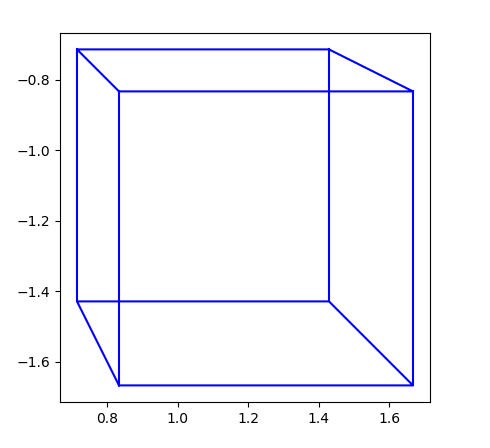
\includegraphics[scale=\myscale,scale=0.25]{ecran-perspective-6-5}
		
		$f=5$
	\end{center}
	\end{minipage}
	\begin{minipage}{0.2\textwidth}
	\begin{center}
		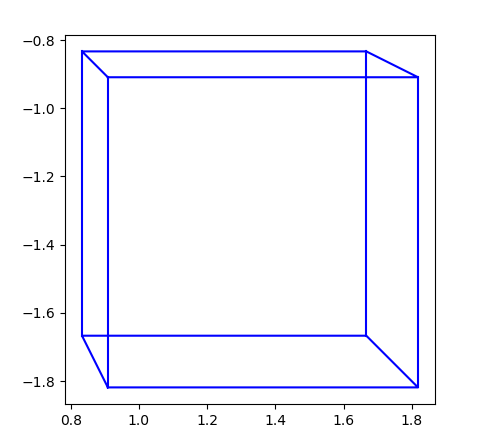
\includegraphics[scale=\myscale,scale=0.25]{ecran-perspective-6-10}
		
		$f=10$
	\end{center}
	\end{minipage}
	\end{center}	
		  
\end{enumerate}
	
\end{activite}


%%%%%%%%%%%%%%%%%%%%%%%%%%%%%%%%%%%%%%%%%%%%%%%%%%%%%%%%%%%%%%%%
%%%%%%%%%%%%%%%%%%%%%%%%%%%%%%%%%%%%%%%%%%%%%%%%%%%%%%%%%%%%%%%%

\begin{cours}[Coordonnées sur la sphère : latitude et longitude]

Pour se repérer dans l'espace on peut utiliser les coordonnées $(x,y,z)$ d'un repère orthonormé direct. Mais pour se repérer à la surface de la Terre ou plus généralement sur une sphère, on peut aussi utiliser les \defi{coordonnées sphériques} $[r :\varphi :\lambda]$ où :
\begin{itemize}
	\item $r>0$ est le rayon de la sphère,
	\item $\varphi$ est la \defi{latitude}, c'est un angle de $[-\frac\pi2,+\frac\pi2]$ (autrement dit compris entre $-90^\circ$ et $+90^\circ$),
	\item $\lambda$ est la \defi{longitude}, c'est un angle de $]-\pi,+\pi]$ (autrement dit compris entre $-180^\circ$ et $+180^\circ$).
\end{itemize}


\myfigure{0.8}{\tikzinput{fig_gps_3d_09}}

\bigskip

\textbf{Passage vers les coordonnées cartésiennes.}

On trouve $(x,y,z)$ en fonction de $[r :\varphi :\lambda]$ par les formules suivantes :
\mybox{
	$\left\{\begin{array}{rcl}
	x & = & r \cos \varphi \cos \lambda \\
	y & = & r \cos \varphi \sin \lambda \\
	z & = & r \sin \varphi
	\end{array}\right.$
}
	
\myfigure{0.7}{\tikzinput{fig_gps_3d_07}}


\bigskip

\textbf{Passage vers les coordonnées sphériques.}

Pour trouver  $[r :\varphi :\lambda]$ à partir de $(x,y,z)$ c'est un peu plus compliqué.

Le rayon 
$$r = \sqrt{x^ 2+y^ 2+z^2}$$

La latitude
$$\varphi = \arcsin \left( \frac{z}{r}\right)$$
La longitude
$$\lambda = \arcsin\left( \frac{1}{\cos\varphi}\frac{y}{r}\right)$$

\end{cours}


%%%%%%%%%%%%%%%%%%%%%%%%%%%%%%%%%%%%%%%%%%%%%%%%%%%%%%%%%%%%%%%%
% Activité 3 - Coordonnées sur la sphère : latitude et longitude
%%%%%%%%%%%%%%%%%%%%%%%%%%%%%%%%%%%%%%%%%%%%%%%%%%%%%%%%%%%%%%%%

\begin{activite}[Coordonnées sur la sphère : latitude et longitude]
	
\index{latitude/longitude}
	
\objectifs{Objectifs : se repérer sur la sphère grâce à la latitude et la longitude.}
	
\begin{enumerate}
		
	\item \textbf{Vers les coordonnées cartésiennes.}
	
	Programme une fonction \ci{latlong_vers_xyz(r,phi,lamb)} qui renvoie les coordonnées
	cartésiennes $(x,y,z)$ du point de coordonnées sphériques $[r:\varphi:\lambda]$.
	
	\emph{Attention.} Ne pas utiliser une variable nommée \ci{lambda} qui est un nom réservé par \Python{} pour autre chose.
	
	\emph{Question.} Quelles sont les coordonnées $(x,y,z)$ du point vérifiant $r=1$, de latitude $\varphi = 45^\circ$ et de longitude $\lambda=30^\circ$. (N'oublie pas de convertir les degrés en radians.)
	
	\item \textbf{Vers les coordonnées sphériques.}
	
	Programme une fonction \ci{xyz_vers_latlong(x,y,z)} qui renvoie les coordonnées sphériques $[r:\varphi:\lambda]$ connaissant ses coordonnées cartésiennes $(x,y,z)$.
	
	\emph{Question.} Quelles sont les coordonnées sphériques $[r:\varphi:\lambda]$ du point $(x,y,z)=(1,2,3)$ ?
	Vérifie que si, à partir de ces $[r:\phi:\lambda]$ et de la première question, tu calcules $(x,y,z)$ tu retrouves bien $(1,2,3)$.
	
	\item \textbf{Tracer les méridiens et les parallèles.}
	\begin{enumerate}
		\item Programme une fonction \ci{trace_meridien(r,lamb)}
		(ou mieux \ci{trace_meridien(r,lamb,nbpoints=100,couleur='red')})
		qui trace le cercle méridien, connaissant le rayon $r$ et la longitude $\lambda$. (Figure de gauche ci-dessous.)
		
		\emph{Indications.}
		\begin{itemize}
			\item Définis $N$ points $[r:\varphi:\lambda]$ où $\varphi$ varie dans $[-\pi,\pi]$.
			\item Calcule les coordonnées $(x,y,z)$ de chacun de ces points.
			\item Relie les points entre eux.
		\end{itemize}
	
	
	\begin{center}
		\begin{minipage}{0.4\textwidth}
			\begin{center}
				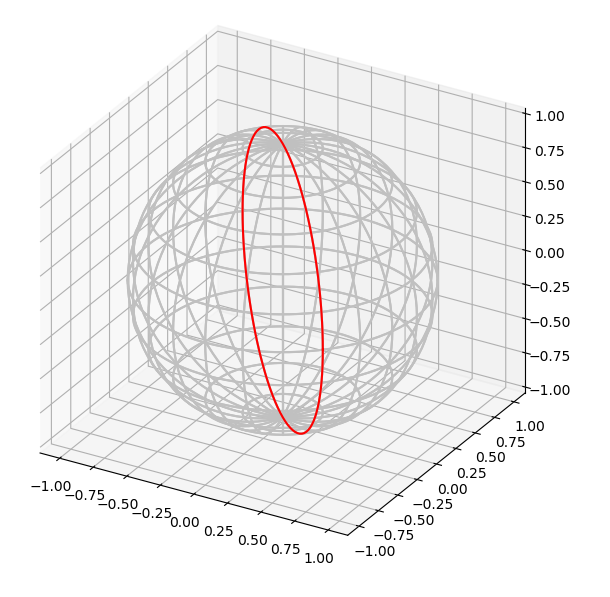
\includegraphics[scale=\myscale,scale=0.3]{ecran-sphere-1new}
				
				\emph{Un méridien.}
			\end{center}
		\end{minipage}
		\begin{minipage}{0.4\textwidth}
			\begin{center}
				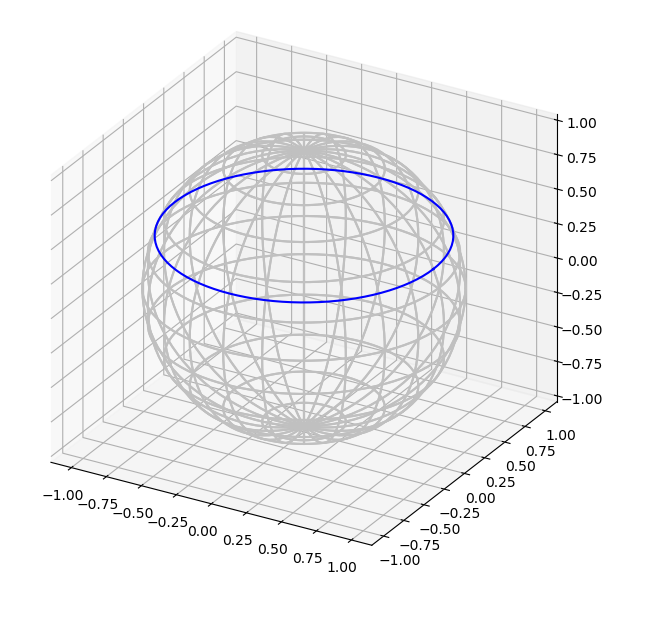
\includegraphics[scale=\myscale,scale=0.3]{ecran-sphere-2new}
				
				\emph{Un parallèle.}
			\end{center}
		\end{minipage}

	\end{center}	
	
	    \item Programme une fonction \ci{trace_parallele(r,phi)}
	    (ou mieux \ci{trace_parallele(r,phi,nbpoints=100,couleur='blue')})
	    qui trace le cercle parallèle, connaissant le rayon $r$ et la latitude $\varphi$. (Figure de droite ci-dessus.)
	    
	    \item  Programme une fonction \ci{trace_meridiens_parallelles(r)}
		qui trace des méridiens et des parallèles sur la sphère de rayon $r$.
				
		\begin{center}
			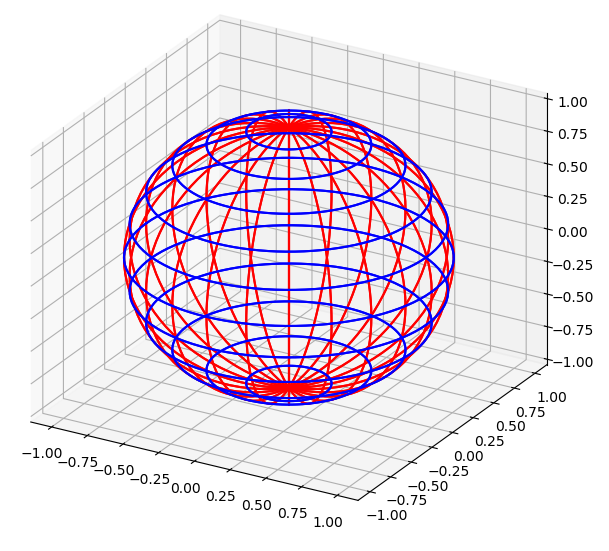
\includegraphics[scale=\myscale,scale=0.3]{ecran-sphere-3}
		\end{center}

	\end{enumerate}

	\item \textbf{Grand cercle passant par deux points.}
	
	\emph{Problème.} Quel est le trajet que doit parcourir un avion entre deux villes de la Terre ?
	
	Mathématiquement, on se donne deux points $P$ et $Q$ sur la sphère de rayon $r$. On cherche le chemin le plus court tracé à la surface de la sphère qui va de $P$ à $Q$. Réponse : c'est un des arcs du \og{}grand cercle\fg{} passant par $P$ et $Q$. Un \emph{grand cercle} est un cercle de rayon $r$ tracé sur la sphère ayant ce même rayon $r$ (l'équateur et les méridiens sont des exemples de grands cercles).
	
	Voici comment tracer ce grand cercle :
	\begin{itemize}
		\item On considère les points $P$ et $Q$ comme des vecteurs : $\vec u = \overrightarrow{OP}$ et 
		$\vec v = \overrightarrow{OQ}$.
		\item On considère le vecteur tournant $\vec{w}(t) = \cos(t)\vec{u}+\sin(t)\vec{v}$, pour $t\in[0,2\pi]$.
		\item On transforme le vecteur $\vec{w}(t)$ en un vecteur de norme $r$ : $\vec{w}'(t) = r \frac{\vec{w}(t)}{\| \vec{w}(t) \|}$.
		\item Le point $R(t)$ à l'extrémité de $\vec{w}'(t)$ est sur le grand cercle passant par $P$ et $Q$ (autrement dit $R(t)$ est tel que $\vec{w}'(t) = \overrightarrow{OR(t)}$).
	\end{itemize}

	Programme une fonction \ci{trace_grand_cercle(P,Q)} qui affiche le grand cercle passant par les deux points $P$ et $Q$.
	
	\begin{center}
	    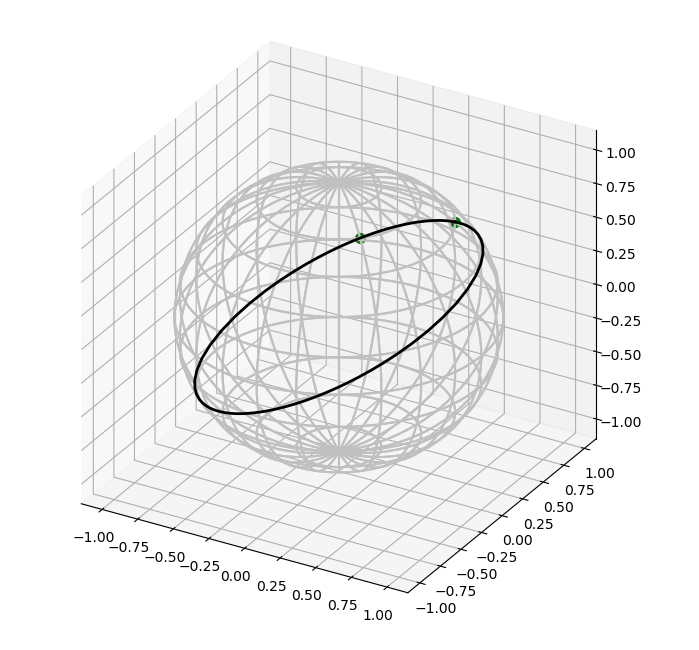
\includegraphics[scale=\myscale,scale=0.3]{ecran-sphere-4newnew}
    \end{center}	
	
\end{enumerate}
	
\end{activite}

%%%%%%%%%%%%%%%%%%%%%%%%%%%%%%%%%%%%%%%%%%%%%%%%%%%%%%%%%%%%%%%%
%%%%%%%%%%%%%%%%%%%%%%%%%%%%%%%%%%%%%%%%%%%%%%%%%%%%%%%%%%%%%%%%

\begin{cours}[Vecteurs]
	
\index{vecteur}
\index{vecteur!produit scalaire}
\index{vecteur!produit vectoriel}


On se place dans un repère orthonormé direct $(O,\vec i,\vec j,\vec k)$. Un vecteur $\vec u$ est représenté par trois coordonnées $(x,y,z)$.

\myfigure{0.8}{\tikzinput{fig-vecteurs-1}} 

Soient $\vec u = (x,y,z)$, $\vec v = (x',y',z')$ deux vecteurs.
\begin{itemize}
	\item \textbf{Addition.} Le vecteur $\vec u + \vec v$ a pour coordonnées $(x+x',y+y',z+z')$.
	
	\item \textbf{Multiplication par un scalaire.} Soit $k\in\Rr$. Alors $k \vec u$ a pour coordonnées
	$(kx,ky,kz)$.
	
	\item \textbf{Produit scalaire.} $\vec u \cdot \vec v = xx'+yy'+zz'$. C'est un nombre réel qui mesure la colinéarité des vecteurs $\vec u$ et $\vec v$.

\myfigure{0.8}{\tikzinput{fig-vecteurs-2}} 
	
	\item \textbf{Norme.} $\| \vec u \| = \sqrt{x^2+y^2+z^2}$. On a aussi $\| \vec u \| =\sqrt{\vec u \cdot \vec u}$. La norme est la longueur du vecteur $\vec u$.
	
	\item \textbf{Vecteurs orthogonaux.} Deux vecteurs  $\vec u$ et $\vec v$ sont orthogonaux si et seulement si $\vec u \cdot \vec v = 0$.
	
	\item \textbf{Angle entre deux vecteurs.}\index{angle}
	La formule suivante permet de calculer l'angle $\theta$ entre deux vecteurs $\vec u$ et $\vec v$ non nuls :
	$$\vec u \cdot \vec v = \| \vec u\| \, \|\vec v\| \cos(\theta)$$
	
	Ainsi 
	$$\theta = \arccos\left(\frac{\vec u \cdot \vec v}{ \| \vec u\| \, \|\vec v\|}\right)$$
	
	\smallskip
	
	\item \textbf{Produit vectoriel.} 
	$\vec u \wedge \vec v$ est le vecteur de coordonnées 
	$$\big(yz'-y'z, zx'-z'x, xy'-x'y \big)$$
	
	Ce vecteur est orthogonal au vecteur $\vec u$ et au vecteur $\vec v$. Autrement dit $\vec w = \vec u \wedge \vec v$ est orthogonal au plan qui contient $\vec u$ et $\vec v$.
	
	
\myfigure{0.8}{\tikzinput{fig-vecteurs-3}} 	
	
	\item \textbf{Produit mixte.}
	C'est le nombre réel associé à trois vecteurs $\vec u$, $\vec v$ et $\vec w$, défini à l'aide d'un produit vectoriel puis d'un produit scalaire :
	$$(\vec u \wedge \vec v) \cdot \vec w$$
				
\end{itemize}	
\end{cours}

%%%%%%%%%%%%%%%%%%%%%%%%%%%%%%%%%%%%%%%%%%%%%%%%%%%%%%%%%%%%%%%%
% Activité 4 - Vecteurs
%%%%%%%%%%%%%%%%%%%%%%%%%%%%%%%%%%%%%%%%%%%%%%%%%%%%%%%%%%%%%%%%

\begin{activite}[Vecteurs]
	
	\objectifs{Objectifs : utiliser les vecteurs pour des calculs dans l'espace.}
	
	\begin{enumerate}
	\item \textbf{Norme et produit scalaire.}
	\begin{enumerate}
		\item Programme une fonction \ci{produit_scalaire(u,v)} qui calcule le produit scalaire de deux vecteurs $\vec u$ et $\vec v$ de $\Rr^3$. La variable \ci{u} contient un triplet \ci{(x,y,z)} représentant les coordonnées de $\vec u$, de même pour \ci{v}.
		
		\item Programme une fonction \ci{norme(u)} qui calcule la norme d'un vecteur $\vec u$ de $\Rr^3$. 
		
		\item Programme une fonction \ci{angle(u,v)} qui calcule l'angle entre des vecteurs $\vec u$ et $\vec v$.
		
		\item Calcule la norme de $\vec u = (1,2,3)$ et de $\vec v = (1,0,1)$. Puis calcule le produit scalaire entre ces deux vecteurs, et enfin l'angle entre ces vecteurs (en radians et en degrés).
		
		
		\item \emph{Application : points visibles ou invisibles.}
		Un observateur regarde dans une direction, selon son champ de vision, quels sont les points visibles ?
			
		\begin{itemize}	
			\item \emph{Modélisation.} L'observateur est au point $O=(0,0,0)$. Il regarde dans la direction $\vec u$. Son champ de vision est déterminé par un angle $\theta$. Sur le schéma ci-dessous le point $P_1$ est visible par l'observateur mais pas le point $P_2$. Bien sûr, dans l'espace, la zone visible est un cône (et pas un secteur comme sur le schéma).
		
			\myfigure{0.7}{\tikzinput{fig-vecteurs-5}}		
		
			\item \emph{Solution.} 
			Un point $P$ est visible depuis $O$ si et seulement si l'angle entre  $\vec u$ et $\overrightarrow{OP}$ est plus petit que $\theta$, c'est-à-dire :
			$$\left| \text{angle}(\vec u,\overrightarrow{OP}) \right| \le \theta$$
			
			\item \emph{Question.} Un observateur a un angle de vision $\theta = 50^\circ$, il regarde dans la direction $(1,1,1)$. Parmi les points 
			$P_1=(1,1,2)$, $P_2=(-1,-1,-2)$, $P_3=(80,10,0)$, $P_4=(85,10,0)$ lesquels sont visibles à ses yeux ?
			
		\end{itemize}		
			
		\item \emph{Application : rebond sur un plan.}
		Une balle arrive sur un plan et rebondit. Quelle est la nouvelle trajectoire de cette balle ?
		
		\begin{itemize}
			\item \emph{Modélisation.} La balle arrive selon un vecteur vitesse $\vec u$, le plan est représenté par un vecteur normal $\vec n$.
			
			\item \emph{Solution.} La balle repart selon le vecteur $\vec v$ qui est un symétrique de $\vec u$ par rapport à $\vec n$ et est donné par la formule suivante :
			on commence par transformer $\vec n$ en un vecteur de norme $1$ :
			$$\vec n' = \frac{\vec n}{\|\vec n\|}$$
			puis on a :
			$$ \vec n = \vec u - 2 (\vec u \cdot \vec n') \vec n'$$
			
			\myfigure{0.8}{\tikzinput{fig-vecteurs-4}}
			
			\item \emph{Question.} Une balle arrive selon le vecteur $\vec u = (1,2,-1)$ et rebondit sur un plan ayant pour vecteur normal $\vec n = (1,1,1)$. Selon quelle direction $\vec v$ repart-elle ?				
		\end{itemize}	
		 
	\end{enumerate} 
	
	\item \textbf{Produit vectoriel.}
	
	\begin{enumerate}
		\item Programme une fonction \ci{produit_vectoriel(u,v)} qui calcule le produit vectoriel entre deux vecteurs $\vec u$ et $\vec v$ de $\Rr^3$. Le résultat est un vecteur $\vec w$ renvoyé sous la forme d'un triplet de coordonnées $(x,y,z)$.
		
		\item Calcule le produit vectoriel $\vec w$ de $\vec u = (1,2,3)$ et $\vec v = (1,0,1)$. Vérifie à l'aide du produit scalaire que $\vec w$ est orthogonal à $\vec u$ et à $\vec v$.
		
		\item \emph{Application : équation d'un plan.} On considère le plan $P$ défini par les trois points $O=(0,0,0)$, $A=(-1,2,5)$, $B = (2,0,3)$. Calcule un vecteur $\vec n = (a,b,c)$ normal à ce plan $P$. Une équation du plan est alors $ax+by+cz=0$.
		
		\item \emph{Application : surface d'un triangle et d'un parallélogramme de l'espace.}
		La surface d'un parallélogramme de l'espace déterminé par deux vecteurs $\vec u$ et $\vec v$ est
		$$S_P = \| \vec u \wedge \vec v \|$$
		La surface du triangle de l'espace déterminé par ces mêmes vecteurs est la moitié :
		$$S_T = \frac 12 \| \vec u \wedge \vec v \|$$
		
		\myfigure{0.8}{\tikzinput{fig-vecteurs-6}}
		
		Calcule la surface du parallélogramme (puis du triangle) déterminé par les vecteurs
		$\vec u = (1,2,-5)$ avec $\vec v = (1,-2,4)$ (il est préférable de donner la réponse à l'aide de la racine carrée d'un entier plutôt qu'une valeur approchée).
		
	\end{enumerate} 		
		
	\item \textbf{Produit mixte.}

	\begin{enumerate}
		\item  Programme une fonction \ci{produit_mixte(u,v,w)} qui calcule le produit mixte de trois vecteurs $\vec u$, $\vec v$, $\vec w$ de $\Rr^3$. On rappelle la formule du produit mixte 
		$$(\vec u \wedge \vec v) \cdot \vec w$$
	
		\item Calcule le produit mixte de $\vec u = (1,2,3)$, $\vec v = (1,0,1)$ et $\vec w = (4,1,0)$.
	
		\item \emph{Application : volume.}
		Le volume d'un parallélépipède de l'espace déterminé par trois vecteur $\vec u$, $\vec v$ et $\vec w$ est
		$$V_P = \big|\text{produit\_mixte}(\vec u,\vec v,\vec w)\big|$$
		Le volume du tétraèdre déterminé par ces mêmes vecteurs est $1/6$ du volume précédent :
		$$V_T = \frac 16 \big|\text{produit\_mixte}(\vec u,\vec v,\vec w) \big|$$
		
		\myfigure{0.5}{\tikzinput{fig-vecteurs-7}}
		
		Calcule le volume du parallélépipède (puis du tétraèdre) déterminé par les vecteurs
		$\vec u = (1,0,0)$, $\vec v = (1,1,0)$ et $\vec w = (1,1,1)$.
		
	\end{enumerate}
\end{enumerate}
	
\end{activite}



%%%%%%%%%%%%%%%%%%%%%%%%%%%%%%%%%%%%%%%%%%%%%%%%%%%%%%%%%%%%%%%%
% Activité 5 - Skyline
%%%%%%%%%%%%%%%%%%%%%%%%%%%%%%%%%%%%%%%%%%%%%%%%%%%%%%%%%%%%%%%%

\begin{activite}[Skyline]
	
	\objectifs{Objectifs : tracer la \emph{skyline} d'une ville, c'est-à-dire le contour apparent de ses gratte-ciels.}
	
	
	Le problème est simple : on souhaite dessiner le contour apparent d'une ville constituée de gratte-ciels.	
\begin{center}
	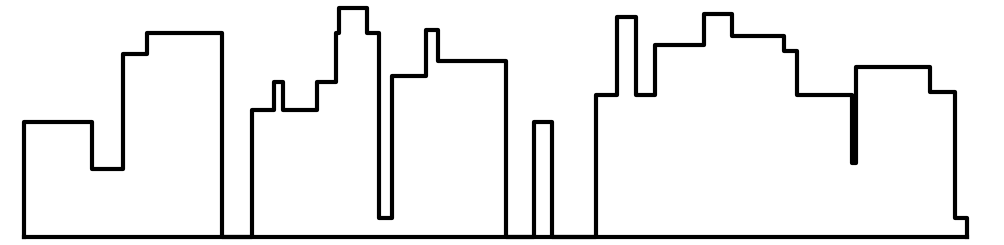
\includegraphics[scale=\myscale,scale=0.3]{ecran-skyline-9}
\end{center}	

  Voici à gauche les immeubles, au centre on dessine le contour, à droite on garde uniquement ce contour.
  
\begin{center}
	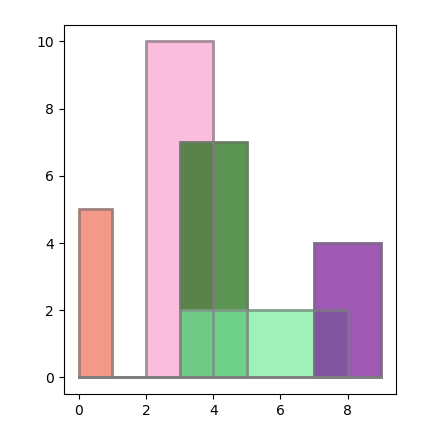
\includegraphics[scale=\myscale,scale=0.3]{ecran-skyline-1}\qquad
	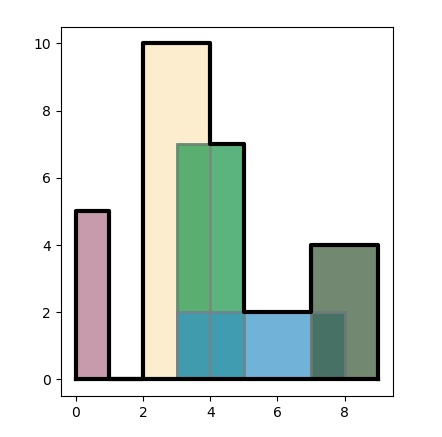
\includegraphics[scale=\myscale,scale=0.3]{ecran-skyline-2}\qquad
	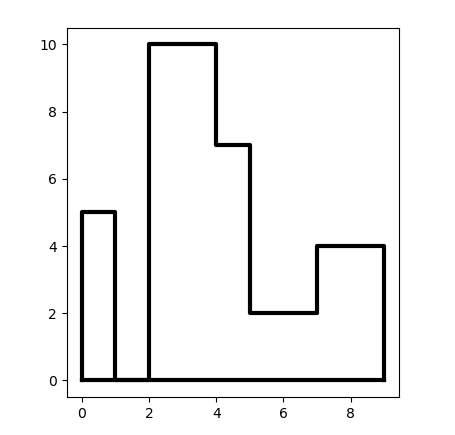
\includegraphics[scale=\myscale,scale=0.3]{ecran-skyline-3}
\end{center}

Voici un autre exemple.

\begin{center}
	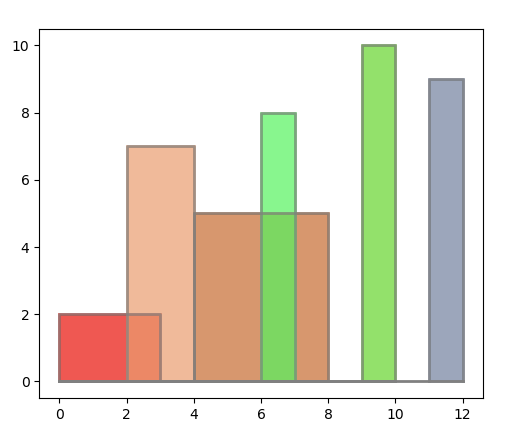
\includegraphics[scale=\myscale,scale=0.25]{ecran-skyline-4}\qquad
	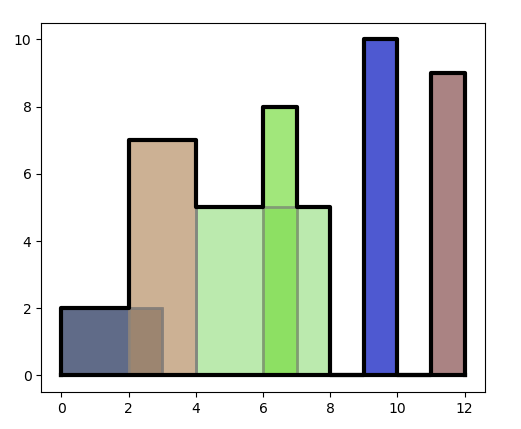
\includegraphics[scale=\myscale,scale=0.25]{ecran-skyline-5}\qquad
	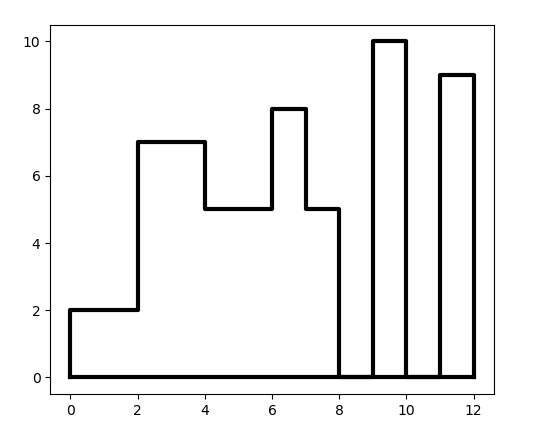
\includegraphics[scale=\myscale,scale=0.25]{ecran-skyline-6}
\end{center}

\bigskip

Ce qui serait formidable c'est de ne pas lire la suite de l'activité et que tu te débrouilles tout seul pour modéliser et résoudre ce problème !

\bigskip

\emph{Indications.} 
\begin{itemize}
	\item Il faut d'abord comprendre que ce problème, qui devrait être un problème en trois dimensions, se ramène à un problème à deux dimensions seulement : qu'un immeuble soit devant ou derrière un autre ne change pas le contour.
	
	\item Il faut aussi avoir conscience que même si le problème est facile à énoncer, trouver une solution n'est pas simple !
	
	\item C'est plus important que tu trouves un algorithme seul, même si il n'est pas parfait, plutôt que de suivre la solution proposée ci-dessous qui est assez optimale.
\end{itemize}


\bigskip	
	
\textbf{Modélisation.}

\begin{itemize}
	\item On modélise un gratte-ciel par un triplet $(x,y,h)$ où $x$ est l'abscisse du côté gauche de l'immeuble, $y$ est l'abscisse du côté droit, $h$ est sa hauteur.
	
	\myfigure{0.4}{\tikzinput{fig-skyline-1}}
	
	\item Une ville est donc une liste d'immeubles. Voici l'exemple pour cette activité :
	\mycenterline{\ci{immeubles = [(0,1,5), (2,4,10), (3,5,7), (3,8,2), (7,9,4)]}}
	
	\begin{center}
		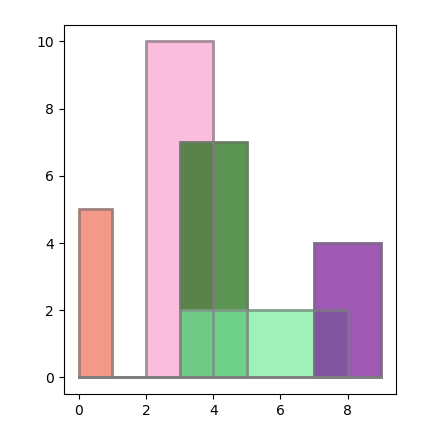
\includegraphics[scale=\myscale,scale=0.4]{ecran-skyline-1}\qquad
	\end{center}
	
\end{itemize}




\bigskip	

\textbf{Principe.} L'idée mise en \oe uvre ci-dessous est la suivante. 
\begin{itemize}
	\item Tout d'abord on récupère tous les bords : ce sont les $x$ ou $y$ correspondant à un côté d'immeuble. 
	
	\item Pour chacun de ces bords, on associe la liste des immeubles qui commencent ou finissent ici. On utilisera un dictionnaire.
	
	\item Pour calculer la \emph{skyline}, on parcourt les bords de la gauche vers la droite. On calcule les listes de tous les immeubles actifs : ce sont les immeubles présents à cette abscisse. 

	\item Chaque bord détermine donc la hauteur maximale actuelle. Si cette hauteur diffère de celle du bord précédent, on a un point de la \emph{skyline} !
	
\end{itemize}

\bigskip	

Voici le travail décomposé en étapes.

\begin{enumerate}
		
	\item Programme une fonction \ci{hauteur_max_immeubles(immeubles)} qui renvoie la hauteur maximale d'une liste d'immeubles (ou $0$ si la liste est vide). 
	
	Par exemple avec :	
	\mycenterline{\ci{immeubles = [(0,1,5), (2,4,10), (3,5,7), (3,8,2), (7,9,4)]}}
	la fonction renvoie la hauteur maximale $h=10$.
		
	\item Programme une fonction \ci{calcul_bords(immeubles)} qui renvoie la liste de tous les bords : dans l'ordre croissant et sans redondance. Un \emph{bord} est une abscisse $x$ ou $y$ d'un immeuble. 
	
	Par exemple avec :	
	\mycenterline{\ci{immeubles = [(0,1,5), (2,4,10), (3,5,7), (3,8,2), (7,9,4)]}}
	la fonction renvoie la liste :	
	\mycenterline{\ci{[0, 1, 2, 3, 4, 5, 7, 8, 9]}}
	
	\item Programme une fonction \ci{dictionnaire_bords_immeubles(immeubles)} qui renvoie un dictionnaire associant à chaque abscisse la liste des numéros d'immeubles ayant un bord ici. Une clé est donc un bord, la valeur une liste de numéros d'immeubles.
	
	Par exemple avec :
	\mycenterline{\ci{immeubles = [(0,1,5), (2,4,10), (3,5,7), (3,8,2), (7,9,4)]}}
	la fonction renvoie le dictionnaire :	
	\mycenterline{dico = \ci{\{0: [0], 1: [0], 2: [1], 4: [1],}} 		
	\mycenterline{{3: [2, 3], 5: [2], 8: [3], 7: [4], 9: [4]\}}}
	
	Par exemple \ci{dico[2]} vaut $[1]$ cela signifie que seul l'immeuble numéro $1$ a un bord à l'abscisse $2$. Autre exemple \ci{dico[3]} vaut \ci{[2, 3]}, cela veut dire que les immeubles numéros $2$ et $3$ ont un bord à l'abscisse $3$.
	
	\emph{Indications.}
	\begin{itemize}
		\item La manipulation d'un dictionnaire est expliquée dans la fiche \og{}Le mot le plus long\fg{}.
		\item Pars d'un dictionnaire vide \ci{dico = \{\}}.
		\item Pour chaque immeuble récupère les valeurs $x$  et $y$ :
		\begin{itemize}
			\item si $x$ n'est pas déjà une clé (test \og{}\ci{x not in dico}\fg{}) crée une nouvelle liste contenant le numéro de l'immeuble (\ci{dico[x] = [i]}),
			\item si $x$ est déjà une clé (test \og{}\ci{x in dico}\fg{}) ajoute le numéro de l'immeuble à la liste (\ci{dico[x].append(i)}),
			\item fais la même chose avec $y$.
		\end{itemize}
		
	\end{itemize}


	\item Programme une fonction \ci{calcul_skyline(immeubles)} qui renvoie la liste des points formant le contour. Pour l'exemple  des questions précédentes le contour est : 
	\mycenterline{\ci{[(0, 0), (0, 5), (1, 5), (1, 0), (2, 0), (2, 10), (4, 10),}} 	
	\mycenterline{\ci{(4, 7), (5, 7), (5, 2), (7, 2), (7, 4), (9, 4), (9, 0)]}}
	
	Voici l'algorithme :
	\begin{itemize}
		\item Calculer la liste des bords et le dictionnaire bords/immeubles.
		\item Initialiser une liste vide pour la \emph{skyline} et une pour les immeubles actifs.
		\item Initialiser une hauteur \ci{h_avant} à $0$.
		\item Pour chaque $x$ dans la liste des bords :
		\begin{itemize}
			\item calculer la liste des immeubles actifs (pour chaque $i$ dans \ci{dico[x]} on ajoute ou on retire l'immeuble numéro $i$ s'il est absent ou déjà présent),
			
			\item  calculer la nouvelle hauteur maximale \ci{h_apres} des immeubles actifs,
			
			\item si \ci{h_avant} et \ci{h_apres} diffèrent alors ajouter à la \emph{skyline} les deux points \ci{(x,h_avant)} et \ci{(x,h_apres)},
		
			\item \ci{h_avant} $\leftarrow$ \ci{h_apres}
		\end{itemize}
	\end{itemize}
	
	
	\item Programme enfin l'affichage des immeubles et de la \emph{skyline} !
\end{enumerate}


Voici un exemple généré au hasard. 
\begin{center}
%	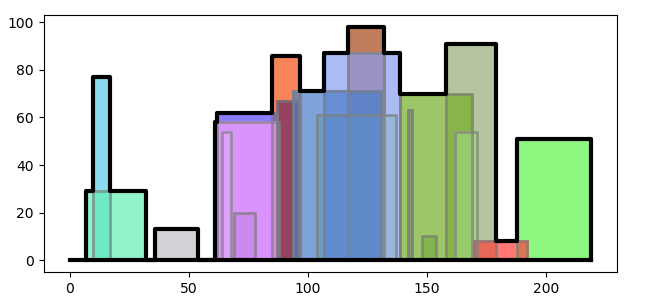
\includegraphics[scale=0.4]{ecran-skyline-7}
	
	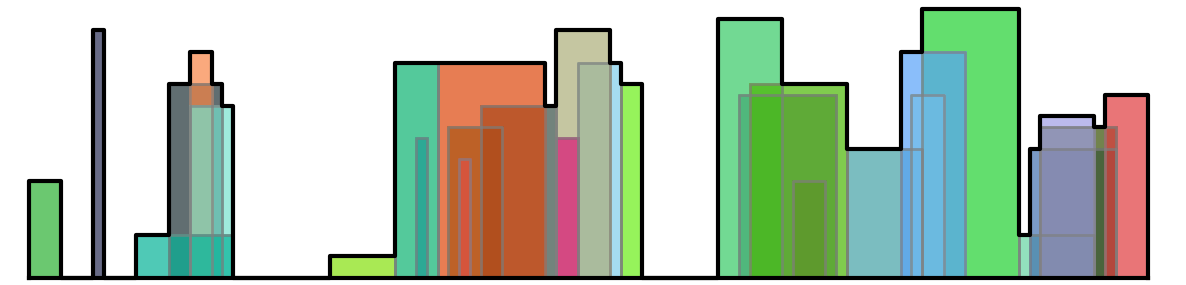
\includegraphics[scale=\myscale,scale=0.4]{ecran-skyline-8}
\end{center}
\end{activite}

\end{document}
